\documentclass[border=2]{standalone}
\usepackage[utf8]{inputenc}

\usepackage{flowchart}
\usetikzlibrary{arrows}

\newcommand{\red}[1]{{\color{red}$#1$}}

\begin{document}
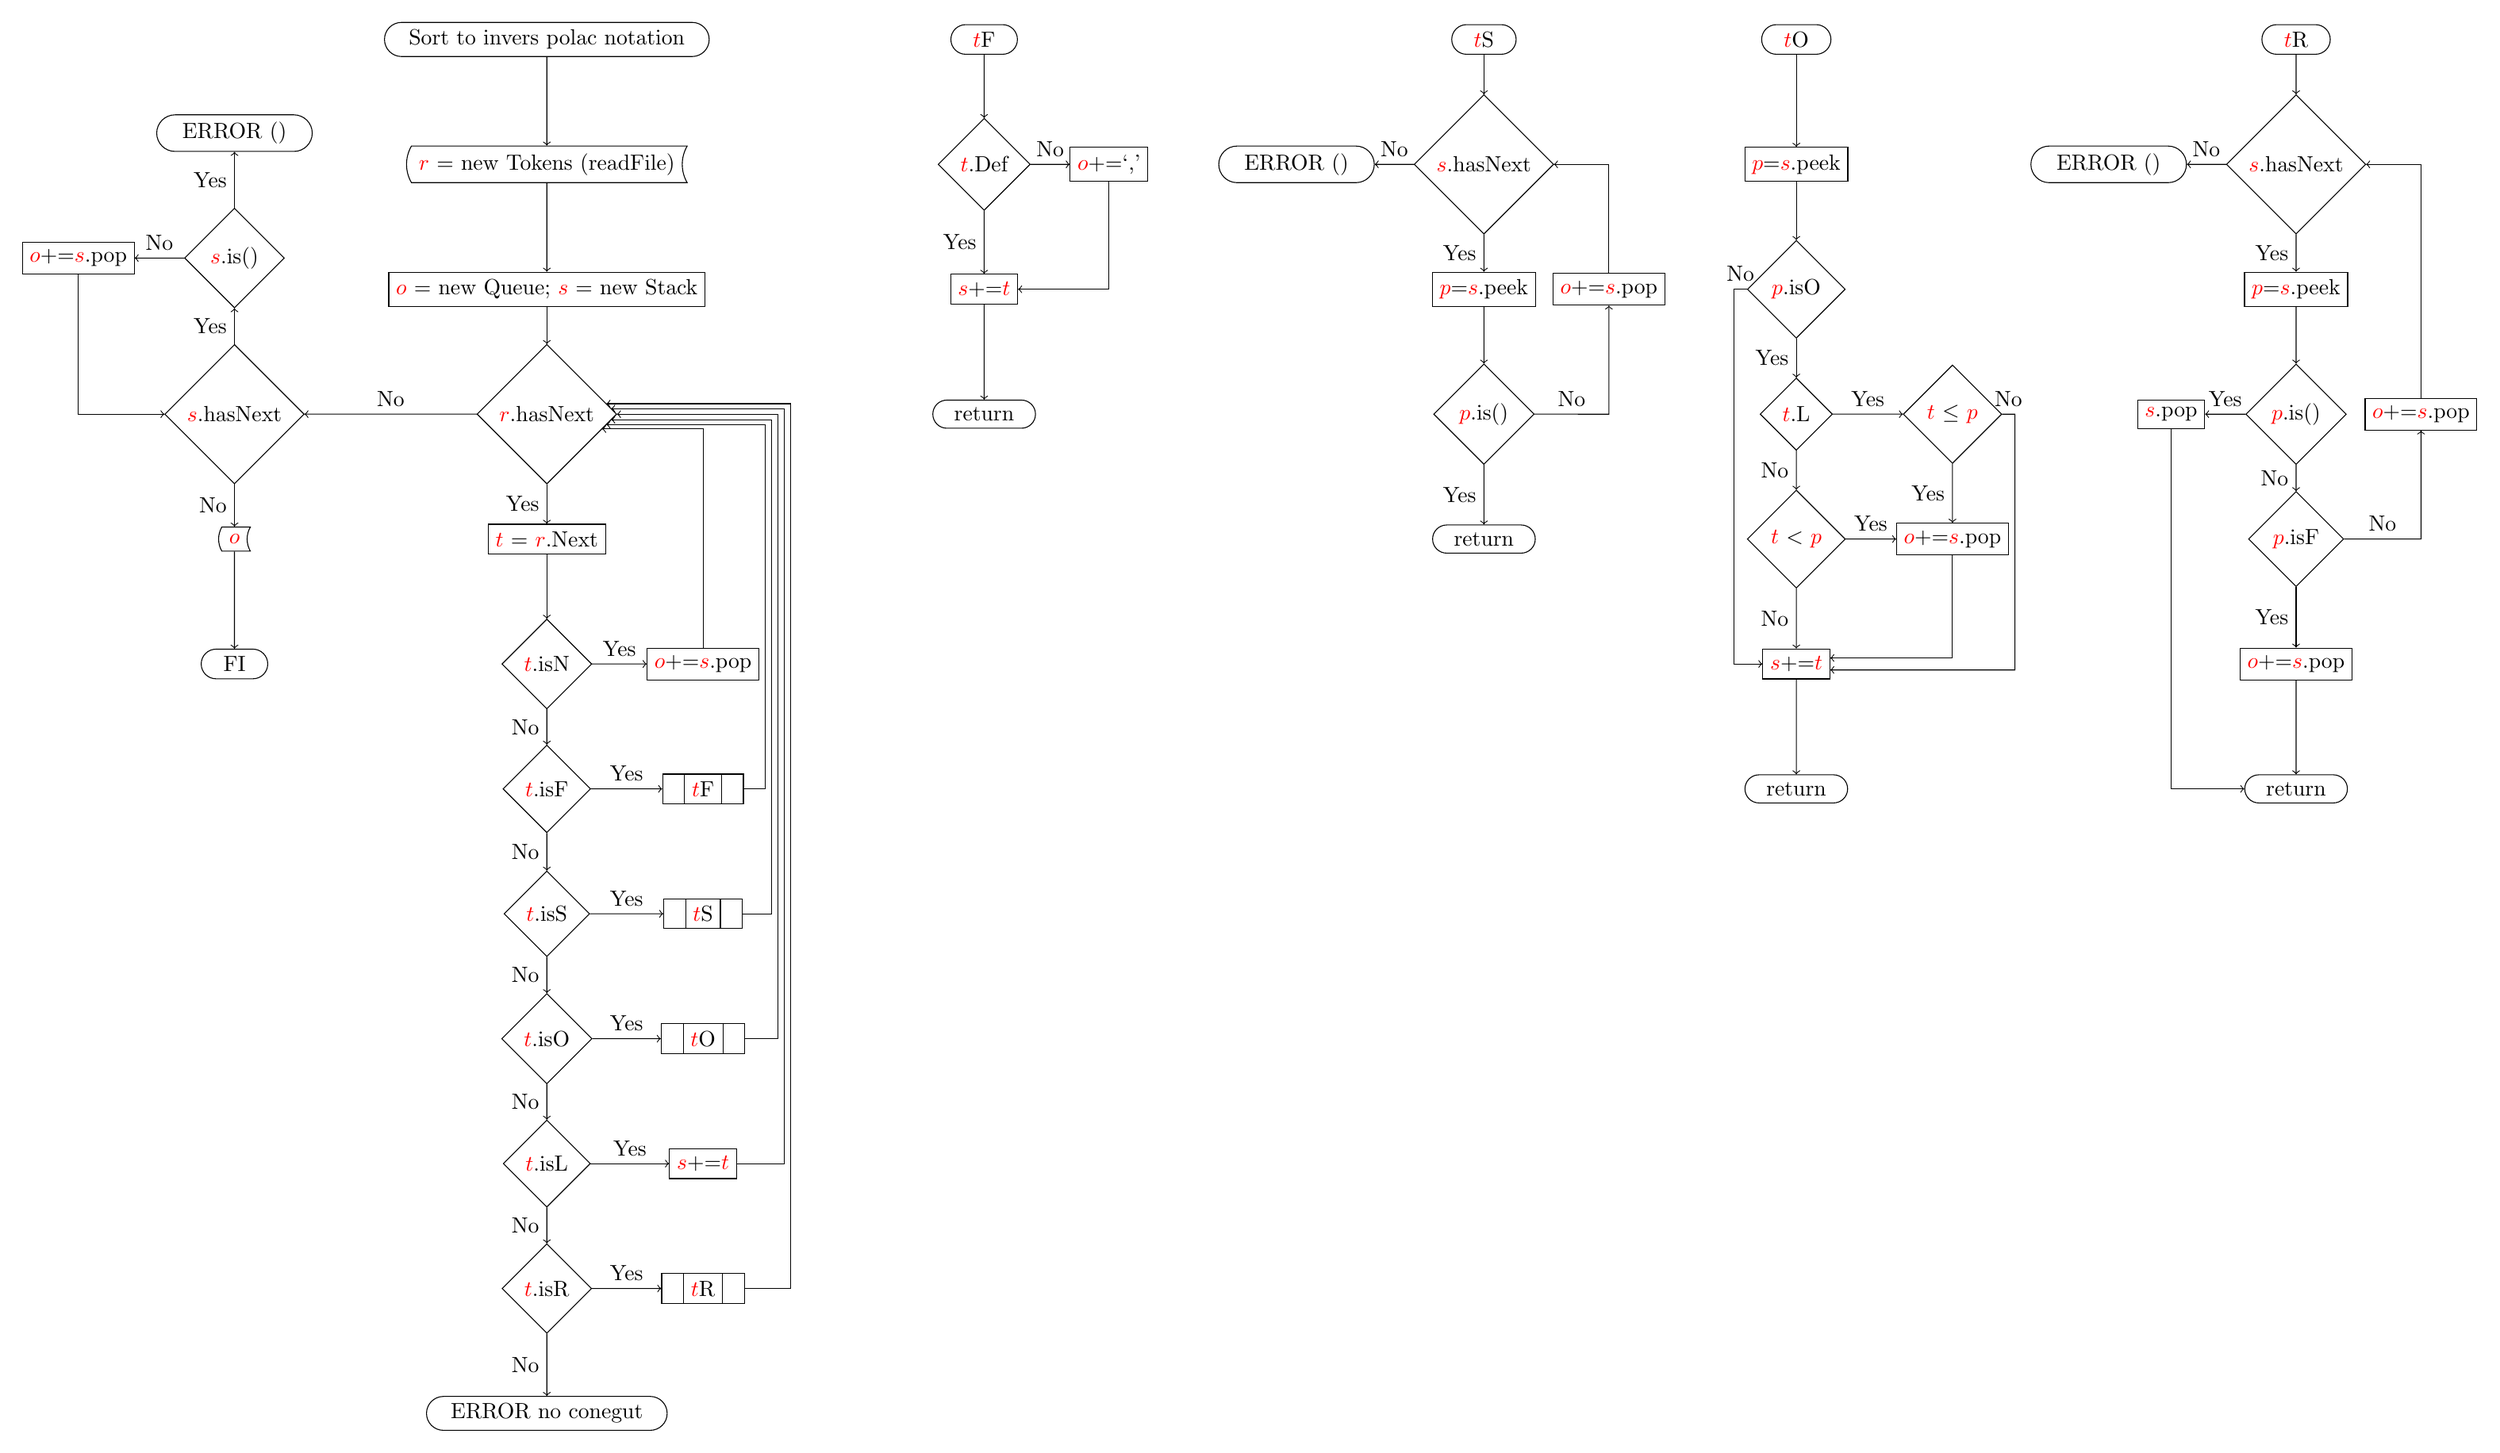
\begin{tikzpicture}[node distance = 2cm, auto]
% process/ decision/ terminal/ predproc/ storage/

%%%%%%%%%%%%%%%%%%%%%%%%%%%%%%%%%%%%%%%%%%%%%%%%%%%%%%%%%%%%%%%%%%%%%%%%%%%%%%%%%%%%%%%%%%%%%%%%%%%%%%%%%%%%%%%%%%%%%%%%%%%%%%%%
% Nucli, principal
%%%%%%%%%%%%%%%%%%%%%%%%%%%%%%%%%%%%%%%%%%%%%%%%%%%%%%%%%%%%%%%%%%%%%%%%%%%%%%%%%%%%%%%%%%%%%%%%%%%%%%%%%%%%%%%%%%%%%%%%%%%%%%%%
\node [draw, terminal] (IniciSatanicContraEvangelics) {Sort to invers polac notation};
\node [draw, storage, below of=IniciSatanicContraEvangelics] (readInfixDirtyNotation) {\red{r} = new Tokens (readFile)};
\node [draw, process, below of=readInfixDirtyNotation] (declareQueueAndStack) {\red{o} = new Queue; \red{s} = new Stack};
\node [draw, decision, below of=declareQueueAndStack] (mainWhile) {\red{r}.hasNext};
	\node [draw, decision, left of=mainWhile, node distance=5cm] (StackEmptyToEnd) {\red{s}.hasNext};
	\node [draw, decision, above of=StackEmptyToEnd, node distance=2.5cm] (StackEndnoLikeParentesis) {\red{s}.is()};
	\node [draw, terminal, above of=StackEndnoLikeParentesis] (ERROREndParentesis) {ERROR ()};
\node [draw, process, left of=StackEndnoLikeParentesis, node distance=2.5cm] (AfegintQuanAsseguratLikeEndParentesis) {\red{o}+=\red{s}.pop};
	\node [draw, storage, below of=StackEmptyToEnd] (GuardantResultat) {\red{o}};
	\node [draw, terminal, below of=GuardantResultat] (FinalEndingPrograma) {FI};
\node [draw, process, below of=mainWhile] (EaserForNotAlotTimePeek) {\red{t} = \red{r}.Next};
\node [draw, decision, below of=EaserForNotAlotTimePeek] (butIsNumber) {\red{t}.isN};
	\node [draw, process, right of=butIsNumber, node distance=2.5cm] (butIsNextNumber) {\red{o}+=\red{s}.pop};
\node [draw, decision, below of=butIsNumber] (butIsFuntion) {\red{t}.isF};
	\node [draw, predproc, right of=butIsFuntion, node distance=2.5cm] (butIsNextFuntion) {\red{t}F};
\node [draw, decision, below of=butIsFuntion] (butIsSeparator) {\red{t}.isS};
	\node [draw, predproc, right of=butIsSeparator, node distance=2.5cm] (butIsNextSeparator) {\red{t}S};
\node [draw, decision, below of=butIsSeparator] (butIsOperator) {\red{t}.isO};
	\node [draw, predproc, right of=butIsOperator, node distance=2.5cm] (butIsNextOperator) {\red{t}O};
\node [draw, decision, below of=butIsOperator] (butIsLeft) {\red{t}.isL};% left parentesis
	\node [draw, process, right of=butIsLeft, node distance=2.5cm] (butIsNextLeft) {\red{s}+=\red{t}};
\node [draw, decision, below of=butIsLeft] (butIsRight) {\red{t}.isR};% right parentesis
	\node [draw, predproc, right of=butIsRight, node distance=2.5cm] (butIsNextRight) {\red{t}R};
\node [draw, terminal, below of=butIsRight] (butIsUnknow) {ERROR no conegut};
\draw[->] (IniciSatanicContraEvangelics)	-- (readInfixDirtyNotation);
\draw[->] (readInfixDirtyNotation)	-- (declareQueueAndStack);
\draw[->] (declareQueueAndStack)	-- (mainWhile);
	\draw[->] (mainWhile)	-- node[anchor=south] {No} (StackEmptyToEnd);
	\draw[->] (StackEmptyToEnd)	-- node[anchor=east] {Yes} (StackEndnoLikeParentesis);
	\draw[->] (StackEndnoLikeParentesis)	-- node[anchor=east] {Yes} (ERROREndParentesis);
	\draw[->] (StackEndnoLikeParentesis)	-- node[anchor=south] {No} (AfegintQuanAsseguratLikeEndParentesis);
		\draw [->] (AfegintQuanAsseguratLikeEndParentesis) |- (StackEmptyToEnd);
	\draw[->] (StackEmptyToEnd)	-- node[anchor=east] {No} (GuardantResultat);
	\draw[->] (GuardantResultat)	-- (FinalEndingPrograma);
\draw[->] (mainWhile)	-- node[anchor=east] {Yes} (EaserForNotAlotTimePeek);
\draw[->] (EaserForNotAlotTimePeek)	-- (butIsNumber);
	\draw[->] (butIsNumber)	-- node[anchor=south] {Yes} (butIsNextNumber);
		\draw[->] (butIsNextNumber)	|- (mainWhile.-15);
\draw[->] (butIsNumber)	-- node[anchor=east] {No} (butIsFuntion);
	\draw [->] (butIsFuntion)	-- node[anchor=south] {Yes} (butIsNextFuntion);
		\draw[->] (butIsNextFuntion)	-- + (1, 0) |- (mainWhile.-10);
\draw[->] (butIsFuntion)	-- node[anchor=east] {No} (butIsSeparator);
	\draw [->] (butIsSeparator)	-- node[anchor=south] {Yes} (butIsNextSeparator);
		\draw[->] (butIsNextSeparator)	-- + (1.1, 0) |- (mainWhile.-5);
\draw[->] (butIsSeparator)	-- node[anchor=east] {No} (butIsOperator);
	\draw [->] (butIsOperator)	-- node[anchor=south] {Yes} (butIsNextOperator);
		\draw[->] (butIsNextOperator)	-- + (1.2, 0) |- (mainWhile);
\draw[->] (butIsOperator)	-- node[anchor=east] {No} (butIsLeft);
	\draw [->] (butIsLeft)	-- node[anchor=south] {Yes} (butIsNextLeft);
		\draw[->] (butIsNextLeft)	-- + (1.3, 0) |- (mainWhile.5);
\draw[->] (butIsLeft)	-- node[anchor=east] {No} (butIsRight);
	\draw [->] (butIsRight)	-- node[anchor=south] {Yes} (butIsNextRight);
		\draw[->] (butIsNextRight)	-- + (1.4, 0) |- (mainWhile.10);
\draw[->] (butIsRight)	-- node[anchor=east] {No} (butIsUnknow);
%%%%%%%%%%%%%%%%%%%%%%%%%%%%%%%%%%%%%%%%%%%%%%%%%%%%%%%%%%%%%%%%%%%%%%%%%%%%%%%%%%%%%%%%%%%%%%%%%%%%%%%%%%%%%%%%%%%%%%%%%%%%%%%%
% Is funtion
%%%%%%%%%%%%%%%%%%%%%%%%%%%%%%%%%%%%%%%%%%%%%%%%%%%%%%%%%%%%%%%%%%%%%%%%%%%%%%%%%%%%%%%%%%%%%%%%%%%%%%%%%%%%%%%%%%%%%%%%%%%%%%%%
\node [draw, terminal, right of=IniciSatanicContraEvangelics, node distance=7cm] (InicitF) {\red{t}F};
\node [draw, decision, below of=InicitF] (CondicioDefinit) {\red{t}.Def};
\node [draw, process, right of=CondicioDefinit] (SeparadorFuntion) {\red{o}+=`,'};
\node [draw, process, below of=CondicioDefinit] (SempreFuntion) {\red{s}+=\red{t}};
\node [draw, terminal, below of=SempreFuntion] (RetornFuntion) {return};
\draw [->] (InicitF)	-- (CondicioDefinit);
\draw [->] (CondicioDefinit)	-- node[anchor=east] {Yes} (SempreFuntion);
\draw [->] (CondicioDefinit)	-- node[anchor=south] {No} (SeparadorFuntion);
\draw [->] (SeparadorFuntion)	|- (SempreFuntion);
\draw [->] (SempreFuntion)	-- (RetornFuntion);
%%%%%%%%%%%%%%%%%%%%%%%%%%%%%%%%%%%%%%%%%%%%%%%%%%%%%%%%%%%%%%%%%%%%%%%%%%%%%%%%%%%%%%%%%%%%%%%%%%%%%%%%%%%%%%%%%%%%%%%%%%%%%%%%
% Is Separator
%%%%%%%%%%%%%%%%%%%%%%%%%%%%%%%%%%%%%%%%%%%%%%%%%%%%%%%%%%%%%%%%%%%%%%%%%%%%%%%%%%%%%%%%%%%%%%%%%%%%%%%%%%%%%%%%%%%%%%%%%%%%%%%%
\node [draw, terminal, right of=InicitF, node distance=8cm] (IniciS) {\red{t}S};
\node [draw, decision, below of=IniciS] (isSeparatorEmpty) {\red{s}.hasNext};
\node [draw, process, below of=isSeparatorEmpty] (DefinintLaInocentP) {\red{p}=\red{s}.peek};
\node [draw, decision, below of=DefinintLaInocentP] (preguntantSiEsFinal) {\red{p}.is()};
\node [draw, terminal, below of=preguntantSiEsFinal] (RetornSeparator) {return};
\node [draw, process, right of=DefinintLaInocentP] (IncrementOutputSeparator) {\red{o}+=\red{s}.pop};
\node [draw, terminal, left of=isSeparatorEmpty, node distance=3cm] (FatalErrorParentesis) {ERROR ()};
\draw [->] (IniciS)	-- (isSeparatorEmpty);
\draw [->] (isSeparatorEmpty)	-- node[anchor=south] {No} (FatalErrorParentesis);
\draw [->] (isSeparatorEmpty)	-- node[anchor=east] {Yes} (DefinintLaInocentP);
\draw [->] (DefinintLaInocentP)	-- (preguntantSiEsFinal);
\draw [->] (preguntantSiEsFinal)	-- node[anchor=east] {Yes} (RetornSeparator);
\draw [->] (preguntantSiEsFinal)	-- node[anchor=south] {No} + (2, 0) -| (IncrementOutputSeparator);
\draw [->] (IncrementOutputSeparator)	|- (isSeparatorEmpty);
%%%%%%%%%%%%%%%%%%%%%%%%%%%%%%%%%%%%%%%%%%%%%%%%%%%%%%%%%%%%%%%%%%%%%%%%%%%%%%%%%%%%%%%%%%%%%%%%%%%%%%%%%%%%%%%%%%%%%%%%%%%%%%%%
% Is Operation
%%%%%%%%%%%%%%%%%%%%%%%%%%%%%%%%%%%%%%%%%%%%%%%%%%%%%%%%%%%%%%%%%%%%%%%%%%%%%%%%%%%%%%%%%%%%%%%%%%%%%%%%%%%%%%%%%%%%%%%%%%%%%%%%
\node [draw, terminal, right of=IniciS, node distance=5cm] (IniciO) {\red{t}O};
\node [draw, process, below of=IniciO] (DefinintLaInocentPenOperation) {\red{p}=\red{s}.peek};
\node [draw, decision, below of=DefinintLaInocentPenOperation] (DirecteOperation) {\red{p}.isO};
\node [draw, decision, below of=DirecteOperation] (IsLeftorRight) {\red{t}.L};
\node [draw, decision, right of=IsLeftorRight, node distance=2.5cm] (Comparation) {\red{t} $\leq$ \red{p}};
\node [draw, decision, below of=IsLeftorRight] (Comparation2) {\red{t} $<$ \red{p}};
\node [draw, process, below of=Comparation] (IsBeautifulOperation) {\red{o}+=\red{s}.pop};
\node [draw, process, below of=Comparation2] (SempreOperation) {\red{s}+=\red{t}};
\node [draw, terminal, below of=SempreOperation] (FinalOperation) {return};
\draw [->] (IniciO)	-- (DefinintLaInocentPenOperation);
\draw [->] (DefinintLaInocentPenOperation)	-- (DirecteOperation);
\draw [->] (DirecteOperation)	-- node[anchor=east] {Yes} (IsLeftorRight);
\draw [->] (DirecteOperation)	-- node[anchor=south] {No} + (-1, 0) |- (SempreOperation);
\draw [->] (IsLeftorRight)	-- node[anchor=south] {Yes} (Comparation);
\draw [->] (IsLeftorRight)	-- node[anchor=east] {No} (Comparation2);
\draw [->] (Comparation)	-- node[anchor=east] {Yes} (IsBeautifulOperation);
\draw [->] (Comparation)	-- node[anchor=south] {No} + (1, 0) |- (SempreOperation.-10);
\draw [->] (Comparation2)	-- node[anchor=south] {Yes} (IsBeautifulOperation);
\draw [->] (Comparation2)	-- node[anchor=east] {No} (SempreOperation);
\draw [->] (IsBeautifulOperation)	|- (SempreOperation.10);
\draw [->] (SempreOperation)	-- (FinalOperation);
%%%%%%%%%%%%%%%%%%%%%%%%%%%%%%%%%%%%%%%%%%%%%%%%%%%%%%%%%%%%%%%%%%%%%%%%%%%%%%%%%%%%%%%%%%%%%%%%%%%%%%%%%%%%%%%%%%%%%%%%%%%%%%%%
% Is Right Parentesis
%%%%%%%%%%%%%%%%%%%%%%%%%%%%%%%%%%%%%%%%%%%%%%%%%%%%%%%%%%%%%%%%%%%%%%%%%%%%%%%%%%%%%%%%%%%%%%%%%%%%%%%%%%%%%%%%%%%%%%%%%%%%%%%%
\node [draw, terminal, right of=IniciO, node distance=8cm] (IniciR) {\red{t}R};
\node [draw, decision, below of=IniciR] (isErrorEndingParentesis) {\red{s}.hasNext};
\node [draw, terminal, left of=isErrorEndingParentesis, node distance=3cm] (ERROREndingParentesis) {ERROR ()};
\node [draw, process, below of=isErrorEndingParentesis] (definidedInocentPinParentesis) {\red{p}=\red{s}.peek};
\node [draw, decision, below of=definidedInocentPinParentesis] (IsleftParentesisinParentesis) {\red{p}.is()};
\node [draw, process, left of=IsleftParentesisinParentesis] (Ending01Parentesis) {\red{s}.pop};
\node [draw, process, right of=IsleftParentesisinParentesis] (ContinueParentesis) {\red{o}+=\red{s}.pop};
\node [draw, decision, below of=IsleftParentesisinParentesis] (IsaFuntioninParentesis) {\red{p}.isF};
\node [draw, process, below of=IsaFuntioninParentesis] (TheAddFuntionInParentesis) {\red{o}+=\red{s}.pop};
\node [draw, terminal, below of=TheAddFuntionInParentesis] (ReturnP) {return};
\draw [->] (IniciR)	-- (isErrorEndingParentesis);
\draw [->] (isErrorEndingParentesis)	-- node[anchor=south] {No} (ERROREndingParentesis);
\draw [->] (isErrorEndingParentesis)	-- node[anchor=east] {Yes} (definidedInocentPinParentesis);
\draw [->] (definidedInocentPinParentesis)	-- (IsleftParentesisinParentesis);
\draw [->] (IsleftParentesisinParentesis)	-- node[anchor=south] {Yes} (Ending01Parentesis);
\draw [->] (IsleftParentesisinParentesis)	-- node[anchor=east] {No} (IsaFuntioninParentesis);
\draw [->] (Ending01Parentesis)	|- (ReturnP);
\draw [->] (IsaFuntioninParentesis)	-- node[anchor=east] {Yes} (TheAddFuntionInParentesis);
\draw [->] (IsaFuntioninParentesis)	-- node[anchor=south] {No} + (2, 0) -| (ContinueParentesis);
\draw [->] (TheAddFuntionInParentesis)	-- (ReturnP);
\draw [->] (ContinueParentesis)	|- (isErrorEndingParentesis);

\end{tikzpicture}
\end{document}

Llegenda:
()	Parentesis
o	output
t	token
r	tokens
s	stack
p	peek stack // code less
L	Left parentesis
R	Right parentesis
N	Number
F	Funtion
S	Separator
O	Operation

Per entendre la magia, una funcio acaba sempre amb (, Ex: v(, ve a ser un vector. % fora pensava amb -, v- etc
llavors entent v( com a parentesis obert
	Aquest tindra un valor, igual que +, -, *, ... El qual indicara si es definit o indefinit, el nombre d'elements d'aquest

Exemple
Indefinit (,)
v( 4 , 6 , 7 ) => , 4 6 7 v-
Definit
M2i2( 1 , 4 , 8 , 9 ) => 1 4 8 9 M2i2-
